\chapter{Mathematical Foundations}

\begin{summary}
    This introductory chapter discusses some of the mathematical prerequisites to studying fractals and their geometries. If the topics seem unfamiliar, you may choose to read this chapter first, or it may be more appropriate to visit these topics as they appear throughout the rest of the text. In general, this book assumes the reader has experience up to a first course in calculus. Although, there will be exercises that utilize knowledge from higher mathematics such as multi-variable calculus. These exercises will come with a warning. 
\end{summary}

\section{Methods of Proof}
While scientists justify their hypotheses with scientific experiments, mathematicians justify their claims via rigorous proof. Depending on the claim, different methods of proof are more useful, and in this section, we will explore three such methods and when to use them. The most common technique is creating a \textbf{direct proof}\index{Direct Proof}, a proof that begins by assuming the hypotheses, using relevant definitions and then implements axioms and previously established results to reach the desired conclusion. Here, we present a few common examples. 

\begin{theorem}
    The sum of two odd integers is even
\end{theorem}
This theorem is declaring a universal statement; there is something true about every pair of odd integers. So, we must take two arbitrary elements that are odd and show that the sum is even. Here, we define an odd integer as an integer that can be written in the form $2k+1$ with $k$ an integer. And an even integer is a number that can be written in the form $2k$
 with $k$ an integer. Now let's construct the proof.
 \clearpage
 
 \begin{proof}
    Let $n$ and $m$ be odd integers. This means that they can be written in the form $2a+1$ and $2b+1$, respectively, with $a,b$ integers. Then, $n+m= \linebreak (2a+1)+(2b+1)=2(a+b+1)$. Since $a+b+1$ is an integer, $2(a+b+1)$ is even. Thus, $n+m$ is even by definition. 
\end{proof}

The next example requires a bit more algebra.
\begin{theorem}[Quadratic Equation]
    The values of $x$ that satisfy the equation $ax^2+bx+c=0$ with reals $a,b,c$ and $a\neq 0$ are $x=\Large{\frac{-b\pm\sqrt{b^2 - 4ac}}{2a}}$.
\end{theorem}
\vspace{-3.5mm}
\begin{proof}
    Assume that reals $a,b,c$ with $a\neq 0$ satisfy the equation $ax^2+bx+c=0$. Then we have
    \begin{align*}
        & & ax^2+bx+c &= 0 &\text{(given)}\\
        &\implies & ax^2+bx &= -c &\text{(subtracting $c$ from both sides)}\\
        &\implies & x^2 + \frac{b}{a}x &= \frac{-c}{a} &\text{(dividing)}\\
        &\implies & x^2 + \frac{b}{a}x + \left(\frac{b}{2a}\right)^2 &= \frac{-c}{a} + \left(\frac{b}{2a}\right)^2 &\text{(adding a term to both sides)}\\
        &\implies & \left(x + \frac{b}{2a}\right)^2 &= \frac{-c}{a} + \frac{b^2}{4a^2} &\text{(factoring the square)}\\
        &\implies & x + \frac{b}{2a} &= \pm\sqrt{\frac{-c}{a} + \frac{b^2}{4a^2}} &\text{(taking the square root)}\\
        &\implies & x &= \frac{-b}{2a} \pm\sqrt{\frac{-c}{a} + \frac{b^2}{4a^2}} &\text{(subtracting from both sides)}\\
        &\implies & x &= \frac{-b}{2a}\pm \frac{\sqrt{b^2-4ac}}{|2a|} &\text{(simplifying the square root)}\\
         &\implies & x &= \frac{-b}{2a}\pm \frac{\sqrt{b^2-4ac}}{2a} &\text{(since $\pm|a|=\pm a$)}\\
        &\implies & x &= \frac{-b\pm\sqrt{b^2 - 4ac}}{2a} &\text{(combining fractions)}
    \end{align*}
\end{proof}

Generally speaking, reading these direct proofs is straight forward. It is usually pretty clear what axioms or theorems we may assume, so we use these like puzzle pieces to generate a proof. It should also be clear by reading the proof how the sequence of steps fit together logically to produce the desired result. \\


\clearpage
However, sometimes it is challenging, or even impossible to find a way to do this. There are many cases where it is easier to prove a claim by assuming the contrary and showing that doing so produces a contradiction or logical fallacy. This is called a \textbf{proof by contradiction}\index{Proof by contradiction}. \\

\begin{theorem}
    There are infinitely many primes.
\end{theorem}
\vspace{-3.5mm}
\begin{proof}
    Assume the contrary, that there are finitely many primes $p_1, p_2, \cdots, p_z$ with $p_z$ being the largest prime. Now, consider the number $n=p_1p_2\cdots p_z +1$. This number is clearly larger than $p_z$, and it must also be divisible by some prime, say $p_i$ (this is a result of the fundamental theorem of arithmetic). We know that $p_i$ divides the quantity $p_1p_2\cdots p_i\cdots p_z$, so it must also divide $n-(p_1\cdots p_z)$. Observe that $n-(p_1\cdots p_z)=1$, so that $p_i$ divides 1, a contradiction.  
\end{proof}

Sometimes, these proofs seem a little bit like black magic; it is not blatantly obvious how our method of argument shows the theorem to be true. But by assuming our claim is false, we eventually came to a contradiction which indirectly shows that our claim must be true. Here is another classic example:

\begin{theorem}
    $\sqrt{2}$ is irrational.
\end{theorem}
\vspace{-3.5mm}

\begin{proof}
    Assume instead that $\sqrt{2}$ is rational, and thus can be written in the form $\frac{p}{q}$ with $p$ and $q$ relatively prime integers with $q\neq 0$. Then, it follows that $\sqrt{2}=\frac{p}{q}\implies 2q^2=p^2$. Since the left side of the equation is even, the right side must be as well. This implies that $p$ is even (Why?). In this case, the right side of the equation must moreover be a multiple of 4, since squaring an even number gives this result. Thus, $q$ must be even. But if both $p$ and $q$ are even, then they are not relatively prime integers, a contradiction. 
\end{proof}

On the discussion of indirect proofs, when trying to prove a statement in the form ``if $p$, then $q$'' (or in logic notation $p\implies q$), it is occasionally easier to instead show ``if $q$ is false, then $p$ is false'' $(\sim q\implies \sim p)$. These two statements are logically equivalent. This is called the \textbf{law of the contrapositive} since $p\implies q$ and $\sim q \implies \sim p$ are \textbf{contrapositives} of each other. There will soon be a few examples where this is relevant (such as Theorem 0.2.1). \\

One last method of proof we will discuss is \textbf{mathematical induction}\index{Mathematical induction} which is often useful when trying to show some propositional function $P(n)$ is true for all natural numbers. These proofs contain two primary parts; showing that $P(1)$ is true (or whatever the least natural number in the particular instance is), and then showing that $P(k)$ being true implies $P(k+1)$ istrue as well. In other words, this shows that $P(n)$ is true for all $n\geq 1$. Let's look at some examples. 

\begin{theorem}
    The sum $1+2+\cdots +n=\frac{n(n+1)}{2}$ for $n\geq 1$
\end{theorem}
\vspace{-4mm}
\begin{proof}
    We will first show that this formula is true for $n=1$. Our sum on the left hand side would simply be $1$, and $\frac{n(n+1)}{2}=\frac{2}{2}=1$ on the right hand side as well. Now for the inductive case, assume that $1+2+\cdots +k=\frac{k(k+1)}{2}$ for some $k\geq 1$. Then, adding $k+1$ to both sides yields the following:
    \begin{align*}
       1+2+\cdots +k+(k+1)&=\frac{k(k+1)}{2}+(k+1) &\text{(addition postulate)} \\
         &=\frac{k(k+1)}{2} +\frac{2(k+1)}{2} &\text{(rewriting as fraction)}\\
         &=\frac{k(k+1)+2(k+1)}{2}  &\text{(combining fractions)}\\
         &=\frac{(k+1)(k+2)}{2}  &\text{(factoring)}\\
    \end{align*}
    This final expression is equal to $\frac{n(n+1)}{2}$ when $n=k+1$. (We have shown that if the formula works for some $k\geq 1$, then it works for $k+1$). Thus, the formula holds for any natural number. 
\end{proof}

Usually, the base case is straightforward, and the inductive case that follows requires more work. Although this is not always the case. Let's try another example, one that is quite breezy and smooth!



\begin{theorem}
    The sum of the first $n$ odd numbers is $n^2$
\end{theorem}

\vspace{-4mm}
\begin{proof}
    We first need to render the statement into a mathematical equation to prove. The $n$-th odd number is $2n-1$, so the statement of the theorem is equivalent to $\sum_{i=1}^n 2i-1 = n^2$. For the base case, observe that when $n=1$, we have $2(1)-1 = 1^2$ which is indeed true. For the inductive case, first assume $\sum_{i=1}^k 2i-1 = k^2$ for some $k\in\N$. Then to get to $n=k+1$, we must simply add $2(k+1)-1$ to both sides. This yields the following:
    \begin{align*}
        \sum_{i=1}^{k} (2i-1)\ + 2(k+1)-1 &= k^2 + 2(k+1)-1 \\
        \sum_{i=1}^{k+1} (2i-1) &= k^2 + 2k + 1 \\
        \sum_{i=1}^{k+1} (2i-1) &= (k+1)^2
    \end{align*}
    The last equation tells us that the sum of the first $k+1$ odd numbers is $(k+1)^2$ as desired. Thus the statement to prove holds for all natural numbers. 
\end{proof}

Now do these exercises as practice! Take a look at each one, and before beginning, determine which of the three methods may be most appropriate to utilize. If you ever come to a dead end, don't be discouraged; search for a new route if that is the case.

\begin{exercise}
    Prove that $x^m$ is non-negative when $x$ is real and $m$ is a positive, even integer.
\end{exercise}
\vspace{-5mm}
\begin{exercise}
    The sum of the first $n$ positive odd numbers is $n^2$.
\end{exercise}
\vspace{-5mm}
\begin{exercise}[Calculus]
    Prove $\frac{d}{dx} x^n = nx^{n-1}$ for integers $n\geq 1$.
\end{exercise}
\vspace{-5mm}
\begin{exercise}
    Prove that $\sqrt[3]{3}$ is irrational.
\end{exercise}
\vspace{-5mm}
\begin{exercise}
    Show that for a positive integer $n$, it follows that $\sum_{i=1}^n i^3 = \left(\sum_{i=1}^n i\right)^2$.
\end{exercise}
\vspace{-5mm}
\begin{exercise}
    Prove that there is a unique solution to $4x-3=13$. (Don't forget the ``unique'' part of your proof!)
\end{exercise}
\vspace{-5mm}
\begin{exercise}
    If, for integers $x$ and $y$, $x^2+y^2$ is even, is it necessarily the case that $x+y$ is also even? 
\end{exercise}
\vspace{-5mm}
\begin{exercise}[The Binomial Theorem]
    For a positive integer $n$ and real numbers $x$ and $a$, it follows that $(x+a)^n=\sum_{r=0}^n \frac{n!}{(n-r)!r!} x^r a^{n-r}$.
\end{exercise}
\vspace{-5mm}
\begin{exercise}
    Find all functions $f : \N\to\N$ such that $$xf(y)+yf(x)=(x+y)f(x^2+y^2)$$
    Here, $\N$ represents the set of natural numbers
\end{exercise}
\vspace{-5mm}
\begin{exercise}
    Prove that 13 divides $2^{4n+2}+3^{n+2}$ for all natural numbers $n$.
\end{exercise}
\vspace{-5mm}
\begin{exercise}
    Suppose we have an infinite set of points in the plane, and the distance between any two is always an integer. Show that all the points are collinear. 
\end{exercise}

\clearpage

\section{Set Theory}

\subsection{Set Notation}


Now we will discuss the notations regarding sets that will be used throughout this text. A \textbf{set}\index{Set} is an unordered collection of objects, which we individually call \textbf{elements}\index{Elements}.  It is standard to use upper-case letters to symbolize sets, just as lower-case letters are used as variables for values. For example, we can write the set $A=\{0, 1, 2\}$. Sets are well-defined, meaning that everything is either an element of the set, or not an element of the set. To say that $2$ is an element of $A$, we may write $2\in A$. Since $4$ is not in the set, we say $4\notin A$. The set that has no elements is called the \textbf{empty set}\index{Empty Set}, symbolized as $\varnothing$ or $\{\, \}$.\\

We often use symbols to represent certain notably important sets. In this text, $\mathbb{N}=\{1,2,3,\cdots\}$, $\mathbb{Z}=\{\cdots, -3, -2, -1, 0, 1,2,3,\cdots\}$, $\mathbb{Q}$ represents the rational numbers $\left\{\frac{p}{q}\ :\ p,q\in\mathbb{Z}\text{ and } q\neq 0\right\}$, and $\mathbb{R}$ signifies the real numbers. On some occasions, we reference the complex numbers as $\mathbb{C}$. \\

The set $A=\{0,1,2\}$ has three elements, so its \textbf{cardinality}\index{Cardinality} is 3. In set notation, we write $\#(A)=3$ to signify this. For finite sets, the cardinality is simply the number of distinct elements. So, $\#(\{0,e,\pi,1,e,\pi\})=4$. For infinite sets, things obviously become more complicated. So we instead define two sets $A$ and $B$ to have equal cardinality if there is a bijective function $f\ :\ A\to B$, that is, every element of $B$ has exactly one element of $A$ that maps to it. \\

\begin{exercise}
    With $a,b,c,d$ all unequal, prove that $\#(\{a,b,c,d\})  = \#(\{3,6,9,12\})$ by creating a bijective function that maps one set to the other. 
\end{exercise}
\vspace{-5mm}
\begin{exercise}
    Show that the even integers $2\mathbb{Z}$ have the same cardinality as the integers $\Z$. 
\end{exercise}

To many students' surprise, $\N$ and $\Q$ have the same cardinality. However, $\#(\R) > \#(\Q)$. Sets like $\N$, $\Z$, and anything else bijective to them are called \textbf{countably infinite}\index{Countably Infinite}. Those whose cardinality is greater are called \textbf{uncountably infinite}\index{Uncountably Infinite}, like $\R$, $\C$, and $\R^n$. It is currently unknown whether or not there exists a set whose cardinality is between these two. Or more formally, it is unknown whether there exists some set $A$ such that $\#(\N)<\#(A)<\#(\R)$. The assumption that no such set exists is called \textbf{the continuum hypothesis}\index{Continuum Hypothesis}. Although, it has been shown that with our usual notions of arithmetic, it is impossible to prove or disprove the hypothesis. This means that using our axioms of arithmetic, the continuum hypothesis may be true or false and not yield any contradictions. \\

\begin{exercise}
    Find a bijective function $f\ : \ \R \to (0,1)$
\end{exercise}
\vspace{-5mm}
\begin{exercise}[Challenge]
    Prove that no bijective function $f\ : \ \Z \to \R$ exists.
\end{exercise}

There are four important binary operations pertaining to sets. First, the \textbf{union}\index{Union} of sets $A$ and $B$, written as $A\cup B$, is a set that contains every element in either $A$ or $B$. So if $A=\{0,1,2\}$ and $B=\{0,2,4\}$, then $A\cup B=\{0,1,2,4\}$. Likewise, the \textbf{intersection}\index{Intersection} of sets $A$ and $B$ contains the elements found in both sets. So we write $A\cap B=\{0,2\}$. Thirdly, the \textbf{difference}\index{Difference of sets} $A \setminus B$ is the set of elements in $A$ that are not found in $B$. So $A \setminus B=\{1\}$ and $B \setminus A=\{4\}$. In symbols, we may write that for any sets $A$ and $B$, $A\setminus B=\{x\ :\ x\in A \text{ and } x\notin B\}$, to which we would say ``$A$ minus $B$ is the set of $x$ such that $x$ is in $A$ and $x$ is not in $B$''. And lastly, the \textbf{Cartesian product}\index{Cartesian product} of sets $A$ and $B$, denoted $A\times B$ is the set of all possible ordered pairs of elements from each set. Note that for such ordered pairs, the first element must be in $A$ and the second element must be in $B$. For example, if $A=\{a,b\}$ and $B=\{c,d,e\}$, then $A\times B = \{(a,c),(a,d),(a,e),(b,c),(b,d),(b,e)\}$. \\

\begin{definition}[Cartesian Product]
    Given sets $A$ and $B$, the \textbf{cartesian product}\index{Cartesian Product}  $A\times B = \{(a,b)\ :\ a\in A, b\in B\}$. $A\times B$ is the set of all possible $(a,b)$ where $a$ is in $A$ and $b$ is in $B$.
\end{definition}

\begin{exercise}
    What do you notice about the cardinalities of $X$, $Y$, and $X\times Y$? Can you create an identity that relates them?
\end{exercise}

To say that $A$ is a \textbf{subset}\index{Subset} of $B$ (or $A\subseteq B$) is to say that every element in $A$ also exists in $B$. Notice that every set is a subset of itself. If $A\subseteq B$ and $B\subseteq A$ for any sets $A$ and $B$, then $A=B$. So, it is usually useful--when attempting to show two sets are equal--to show that they are both subsets of each other. On the other hand, if $A$ is a $\textbf{proper subset}$\index{Proper subset} of $B$, i.e. $A\subset B$, then although every element of $A$ is in $B$, it is NOT the case that every element of $B$ is in $A$. 

\begin{exercise}
    Prove that $(A\setminus B) \cap (B\setminus A) =\varnothing$ for any sets $A$ and $B$. \\ Hint: this may be a good time to practice proof by contradiction.

\end{exercise}


\begin{example}[Showing that $\varnothing\subseteq A$ for any set $A$]
    In logic notation, showing that $S\subseteq T$ for any general sets $S$ and $T$ requires showing, by definition, that $\forall y\in S \implies y\in T$. So for this example investigation, we must show $\forall y\in\varnothing \implies y\in A$. But since $y\in\varnothing$ is false for every $y$ by the definition of $\varnothing$, every implication is true, and therefore $\forall y\in\varnothing \implies y\in B$, vacuously. This is arguably the most efficient way of showing $\varnothing\subseteq A$.
\end{example}

\begin{exercise}
    Prove that $(A\setminus B) \cup (B\setminus A) = (A\cup B) \setminus (A\cap B)$
\end{exercise}
    \vspace{-4mm}
\begin{exercise}
  Let $A = \{1, 2, 3\}$ and $B = \{2, 3\}$.
  Determine the following sets. \\
  (a) $A \cup B$ \quad
  (b) $A \cap B$ \quad
  (c) $A \setminus B$ \quad
  (d) $A \times B$
\end{exercise}
    \vspace{-4mm}
\begin{exercise}
    To say $n\mid m$ means that $m$ is a multiple of $n$, or more formally, $n$ divides $m$. There exists some integer $k$ such that $m=nk$.\\ 
    Prove that $\{x\in\mathbb{Z}\, : \, 2\mid x\}\cap \{x\in\mathbb{Z}\, : \, 9\mid x\}\subseteq \{x\in\mathbb{Z}\ : \ 6\mid x\}$
\end{exercise}
    \vspace{-4mm}
\begin{exercise}
    We define $x\equiv y (mod\, n)$ to mean there exists an integer $k$ such that $x+kn=y$. Show $\{(x,y)\in\mathbb{Z}\times\mathbb{Z}\, : \, x\equiv y (mod\, 6)\}$ is a subset of $\{(x,y)\in\mathbb{Z}\times\mathbb{Z}\, : \, x\equiv y (mod\, 3)\}$
\end{exercise}

\begin{example}
    Suppose $C\neq\varnothing$. Prove that if $A\times C = B\times C$, then $A\subseteq B$. \\
    \begin{proof}
        Let $a\in A$. Since $C\neq\varnothing$, there exists $c\in C$. Thus, we have $(a,c)\in A\times C$, by the definition of the Cartesian product. But granted $A\times C=B\times C$, it follows that $(a,c)\in B\times C$ also. Again by the definition of the Cartesian product, we know $a\in B$. Since we have shown $a\in A$ implies $a\in B$, we know $A\subseteq B$. 
    \end{proof}
\end{example}

\begin{exercise}
    Suppose $C\neq\varnothing$. Prove that if $A\times C = B\times C$, then $A=B$. 
\end{exercise}
\

When we finally introduce the definition of a fractal in this book, it will be clear why we emphasize having the ability to relate sets and geometric objects. We need a way to transform a set into an equivalent geometric object, and vice versa. For example, high school students think of graphing functions in highly geometric terms; the graph of the equation $y=3x+2$ is a straight line. In set notation however, we might instead say the graph of $y=3x+2$ is the set $\{(x,y)\in\R^2\,:\,y=3x+2\}$. It is the set of all points $(x,y)$ that satisfy the given equation. \\

How might we represent all the points that are NOT on the line $y=3x+2$? If we define $S=\{(x,y)\,:\,y=3x+2\}$, then we can write $\R^2 / S$ as the set of all points not on the line. This is the exact same as referring to the \textbf{complement} of $S$, notated as $S^c$. In particular, this refers to every element in some universal set $\U$ that is not in $S$. In order for this notation to work, it must be clear what $\U$ is. Since we defined $S$ as being points in $\R^2$, it is clear that $\R^2$ is our universal set. When it is not clear what $\U$ should be, it is best to use the usual set difference notation, but many times, we will go for the simpler set complement notation. \\

\begin{definition}[Set Compliment]
	For some known $\U$, the compliment of $S$, written $S^c$, is defined as \\$\U / S=\{t\in\U\,:\,t\notin S\}$
\end{definition}\index{Set Compliment}

\begin{theorem}
	For any universal set $\U$ and some set $S\subseteq\U$, it follows $S\cup S^c=\U$
\end{theorem}
\begin{proof}
	\begin{itemize}
		Let $\U$ be given and assume some set $S\subseteq\U$. To show $S\cup S^c=\U$, we will prove $S\cup S^c\subseteq\U$ and $S\cup S^c\supseteq\U$
		\item[$\subseteq$] Let $a\in S\cup S^c$. This means $a\in S$ or $a\in S^c$ must be true. If $a\in S$, then $a\in \U$ because $S\subseteq \U$. If $a\in S^c$, then by definition $a\in \{t\in\U\,:\,t\notin S\}$. As a result, $a\in \U$, showing that every element of $S\cup S^c$ is also an element of $\U$. 
		\item[$\supseteq$] Let $a\in \U$. Because sets are well-defined, it follows that $a\in S$ or $a\notin S$ must be true. If $a\notin S$, then $a\in S^c$. Thus $a\in S$ or $a\in S^c$, showing that $a\in S\cup S^c$. 
	\end{itemize}
\end{proof}

\begin{exercise}
	Prove for any universal set $\U$ and some set $S\subseteq\U$, it follows $S\cap S^c=\varnothing$.
\end{exercise}
    \vspace{-3mm}

\begin{exercise}
	Show $\left(S^c\right)^c = S$. 
\end{exercise}

Remember that sets can contain anything, meaning sets may be collections of other sets. As an example, the \textbf{power set} of some set $S$ is the set of all subsets of $S$. If $S=\{1,2\}$, we may write $\mathcal{P}((\{1,2\})=\{\{\},\{1\},\{2\},\{1,2\}\}$, or more simply, $\mathcal{P}(S)=\{\varnothing,\{1\},\{2\},S\}$. This unary operation on sets will be brought up throughout the book in numerous settings. \\

\begin{definition}[Power Set]
	$\mathcal{P}(S)=\{T\,:\, T\subseteq S\}$. The \textbf{power set} of $S$ is the set of all subsets of $S$. 
\end{definition}\index{Power Set}

\begin{exercise}
	Write out $\mathcal{P}(\{a,b,c\})$.
\end{exercise}
    \vspace{-3mm}

\begin{exercise}
	Prove $\#(\mathcal{P}(S))=2^{\#(S)}$.
\end{exercise}
    \vspace{-3mm}

\begin{exercise}[Challenge]
	Show $\#(\mathcal{P}(\N))=\#(\R)$.
\end{exercise}
\clearpage

\begin{definition}[Disjoint sets]
    Two sets $A$ and $B$ are \textbf{disjoint} if $A\cap B=\varnothing$. This means they share no elements in common.
\end{definition}\index{Disjoint Sets}

\begin{exercise}
    Prove that the sets of even integers and odd integers are disjoint. 
\end{exercise}
    \vspace{-4mm}

\begin{exercise}
    Suppose $\sqrt{2}\Q$ is the set of all $\sqrt{2}r$ where $r\in\Q$. Prove $\sqrt{2}\Q$ and $\Q$ are disjoint. 
\end{exercise}
    \vspace{-4mm}

\begin{exercise}
    If $A$ and $B$ are disjoint and $B$ and $C$ are disjoint, is it the case that $A$ and $C$ are disjoint as well?
\end{exercise}
    \vspace{-4mm}

\begin{exercise}
    If $\#(A)=\#(B)$ and $\#(B)=\#(C)$, is it the case that $\#(A)=\#(C)$?
\end{exercise}

\subsection{Infimum and Supremum}

Suppose we have a set of real numbers: $S=\{0,\frac{1}{2},\frac{2}{3},\frac{3}{4},\cdots\}$. If we were to treat the elements of $S$ as a sequence $s_i$, it would not be hard to see that the values are approaching $1$, i.e. $\lim_{i\to\infty}s_i=1$. And because no value of the sequence passes $1$, we may say that $1$ is an upper bound of $S$. Similarly, $\frac{3}{2}$ is an upper bound of $S$ because no element of $S$ is larger than $\frac{3}{2}$. However, the least upper bound, which we will call the \textbf{supremum}\index{Supremum}, is $1$. We may notate this as $\sup(S)=1$ because $1$ is the smallest real number such that no value of $S$ is greater. \\

Likewise, the \textbf{infimum}\index{Infimum} of a set is the greatest lower bound. And in our case where we defined $S=\{0,\frac{1}{2},\frac{2}{3},\frac{3}{4},\cdots\}$, it is clear that $\inf(S)=0$ because no element of $S$ is lower than $0$, and $0$ is the largest number with this property. Notice that $0$ happens to be the minimum of $S$, but $S$ does not have a maximum. 

  \begin{center}

\begin{wrapfigure}{r}{1\textwidth}
    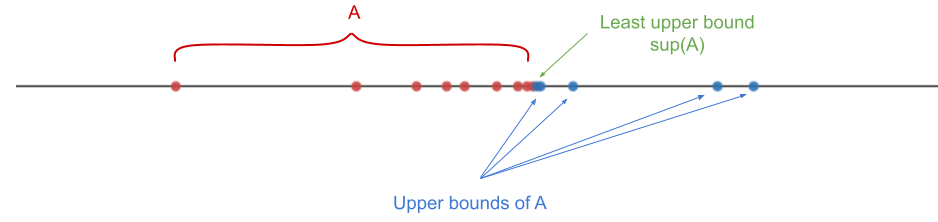
\includegraphics[width=1\textwidth]{Images/Chap0/0sup.png}
  \caption{Geography of the supremum}
\end{wrapfigure}
  \end{center}

\clearpage


In the case that no upper bound or lower bound exists for a set $S$, there does not exist a supremum or infimum (without any upper bounds, a smallest upper bound is impossible). However, if a set is bounded and nonempty, then we are guarateed both an inf and a sup. For example, if we know there exists a lower-bound for a nonempty set, then there must be some ``greatest'' lower-bound. This is known as the \textbf{axiom of choice}\index{Axiom of Choice}, so it is not something to prove here. When trying to show a set has a particular supremum or infimum, we must first show it exists. And to do this, we show that the set is non-empty, and then show that it is bounded in the desired direction (either a lower bound or an upper bound). \\

\begin{example}[Calculating the infimum]
    Let $0<x<1$ and $A=\{x^n\, :\, n\in\mathbb{N}\}$. Show that $\inf(A)=0$.\\

    \begin{proof}
        Since $x\geq 0$, $x^n\geq 0$ for all $n\in\N$. This means that for all $a\in A$, $a\geq 0$, implying $A$ has a lower bound of 0. Also, the set $A$ is not empty, so it follows that $A$ has an infimum by the axiom of choice. Let $\inf(A)=y$ and note that $y\geq 0$. Since $y<x^n$ for $n=0,1,2,\cdots$, we know $y\leq x^{n+1}$ for $n\in\mathbb{N}$, and therefore $\frac{y}{x}\leq x^n$ for $n\in\mathbb{N}$. Thus, $\frac{y}{x}$ is a lower bound for $A$ and $\frac{y}{x}\leq y$. Since $x<1$ and $y\geq 0$, the only way this inequality may hold is when $y=0$.
    \end{proof}
\end{example}

\begin{exercise}
    In the previous example, we concluded that given $\frac{y}{x}\leq y$, $x<1$, and $y\geq 0$, it must follow that $y=0$. Do the algebra on your own to show this by way of contradiction.
\end{exercise}
    \vspace{-3mm}
\begin{exercise}
    In the context of the previous example, find $\sup(A)$. 
\end{exercise}
    \vspace{-3mm}
\begin{exercise}
    Determine (if they exist)  $\sup(S),\inf(S),\max(S),$ and $\min(S)$ if \[S=\left\{x\in\R\ : \ \frac{1}{x-1}>2\right\}\]
\end{exercise}

When it comes to proofs involving the infimum or supremum, we may want to utilize a technique called an $\varepsilon$-proof (epsilon-proof). By saying that $x=\inf(A)$, we declare that there is no lower bound for $A$ greater than $x$. So, if we were to add a very small positive number $\varepsilon$ to $x$, this value would no longer be a lower bound. This brings us to the opportunity to redefine these two set characteristics. \\

\begin{theorem}
    Assume $x$ is a lower bound of $S$. Then, $\inf(S)=x$ if and only if for all $\varepsilon>0$, there exists $s\in S$ such that $s<x+\varepsilon$.
\end{theorem}

We are asked to prove a statement in the form $p\iff q$. Usually this means we prove the statements $p\implies q$ and $q \implies p$. But in our proof, we will choose to prove $p\implies q$ and $\sim p \implies \sim q$ instead. 

\begin{proof}
    ($p\implies q$)\ Assume $\inf(S)=x$. Then, $x+\varepsilon$ cannot be a lower bound for $S$ because there would be an element of $S$ larger than $x+\varepsilon$, a contradiction.\\
   ($\sim p \implies \sim q$)\ Assume $x$ is a lower bound but not the infimum. This implies there is another lower bound $y>x$. Let $\varepsilon=y-x$. Then, there does not exist $s\in S$ such that $s<x+\varepsilon=y$, precisely as desired. 
\end{proof}

\begin{exercise}
    Suppose $A$ has an upper bound of $b$. Prove that $x=\sup(A)$ if and only if $\forall\varepsilon>0,\, \exists s\in S$ such that $s>x+\varepsilon$
\end{exercise}

With these two new formulations of what infimum and supremum mean, many other theorems involving the infimum and supremum may be much easier to resolve. Here are a few, and you will notice it is most appropriate to use the results from Theorem 0.2.2 and Exercise 0.2.24 to solve them. \\

\begin{theorem}
    For some nonempty set $A$, if $\max(A)$ exists, then $\sup(A)=\max(A)$. 
\end{theorem}
\begin{proof}
    Let $A$ be a set with a maximum $a_M$. We know $A$ is nonempty and $a_M$ is an upper bound, thus a supremum exists; call it $s$. Since $a_M\in A$, it follows from the definition of supremum that $s\geq a_M$. Now we will show that $s\leq a_M$. Let $\varepsilon >0$. Granted $\sup(A)=s$, we know there exists $x\in A$ such that $x\geq s-\varepsilon$. Then it follows $a_M \geq s-\varepsilon$.
\end{proof}

\begin{exercise}
    Prove that if $A$ has a minimum, then $\inf(A)=\min(A)$.
\end{exercise}
    \vspace{-4mm}
\begin{exercise}
    Prove that if $\#(A)=1$, then $\inf(A)=\sup(A)$.
\end{exercise}
    \vspace{-4mm}
\begin{exercise}
    Let $S$ be a set with positive elements, and let $T=\left\{\frac{1}{s}\ :\ s\in S\right\}$. Show that $\inf(T)=\frac{1}{\sup(S)}$ 
\end{exercise}
    \vspace{-4mm}
\begin{exercise}
    Suppose $A$ and $B$ are two nonempty sets bounded below. Prove that $\inf(A\cup B)=\min\left\{\inf(A),\inf(B)\right\}$.
\end{exercise}
    \vspace{-4mm}
\begin{exercise}
    Can we say anything about $\inf(A\cap B)$ given each nonempty set is bounded below? Or is there a problem here?
\end{exercise}
    \vspace{-4mm}
\begin{exercise}[Challenge]
    Suppose $A_1,A_2,\cdots$ (countably many) are bounded above. Prove that $\sup(\bigcup_{i=1}^\infty A_i)=\sup\{\sup(A_i)\}$.
\end{exercise}



\clearpage

\section{Metrics and Measures}

\subsection{Metrics}


In everyday life, we measure objects either by size, distance, area, weight, etc. Mathematics provides a way to generalize the notion of ``distance'' between positions in space, or even what it means to ``measure'' objects. First, we will define what it means for a function $d(x,y)$ to be a metric on a set $X$. A metric is another way of referring to a ``distance'' function.\\

Recalling from geometry class, you were likely told that the distance from two points $(x_1,y_1)$ and $(x_2,y_2)$ is given by $\sqrt{(x_2-x_1)^2+(y_2-y_1)^2}$. It is a function that takes in two points and outputs a real number. Or in essence, distance is a function $d$ that maps $\R^2\times\R^2\to\R$. But distance comes with a few particular properties. 

\begin{itemize}
    \item (Identity Property) The distance between any point and itself is $0$.
    \item (Positivity Property) The distance between any two distinct points is positive. 
    \item (Commutative Property) The distance from $A$ to $B$ is the same as the distance from $B$ to $A$.
    \item (Triangle Inequality) The distance from $A$ to $B$ plus the distance from $B$ to $C$ is not less than the distance from $A$ to $C$.
\end{itemize}

All four of these properties should be evidently intuitive, so try the following exercise before moving on.\\

\begin{exercise}
    Render the properties above into formal mathematical statements. And then prove that the standard distance function $\R^2\times\R^2\to\R$ satisfies each of them.
\end{exercise}

Just as it happens in many areas in mathematics, we try to generalize our intuitions about very concrete concepts into more abstract ideas. In fact, there exists a term for any function that obeys these axioms: a metric. So in the previous exercise, you have shown that the distance function is a metric on $\mathbb{R}^2$. The following definition will show how we generalize this notion.\\

\begin{definition}[A Metric on $X$]
    A function $d: X\times X \to \R$ is a metric on $X$ if the following axioms hold for any $x,y,z\in X$:
    \begin{enumerate}
        \item (Identity) $d(x,x)=0$. 
        \item (Positivity) If $x\neq y$, then $d(x,y)>0$. 
        \item (Commutativity) $d(x,y)=d(y,x)$. 
        \item (Triangle Inequality) $d(x,y)+d(y,z)\geq d(x,z)$. 
    \end{enumerate}
\end{definition}\index{Metric}
\vspace{3mm}

The first three axioms are certainly obvious for our example of distance. But the triangle inequality naturally arises from the notion of distance as well. To get from $x$ to $z$, you make take as long as you would like to get there, adding detours to pass through $y$, but doing so will be no shorter in distance than going directly from $x$ to $z$ in a straight line. \\

\begin{definition}[A Metric Space]
    By treating a set and a metric on the set as one object, we produce a \textbf{metric space}. For example, by letting $d_1$ represent Euclidean distance, $(\R^2,d_1)$ is a metric space.
\end{definition}\index{Metric space}
\vspace{3mm}


\begin{wrapfigure}{r}{0.5\textwidth}
  \begin{center}
    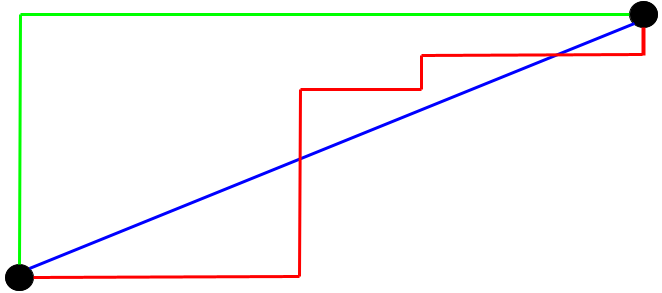
\includegraphics[width=0.45\textwidth]{Images/Chap0/metrics.png}
  \end{center}
  \caption{Given two points, the Euclidean distance (blue) versus the taxicab distance (red or green). Both the red and green paths have the same distance.}
\end{wrapfigure}

Notice that from our definition, a metric doesn't necessarily have to be the distance function. Although Euclidean distance in $\R^2$ (which we will now denote $d_1$) is a convenient example, there are plenty of other functions that satisfy the four given axioms. The Manhattan metric (or sometimes called the taxicab metric) is defined as follows: given two points $(x_1,y_1)$ and $(x_2,y_2)$ in $\R^2$, the taxicab metric $(d_2)$ is $|x_2-x_1|+|y_2-y_1|$. It gets its name because it is the distance between two points if you are only able to travel directly north or south, and east or west, as one would in a taxicab. \\

The image above shows what this may look like. It is the distance needed to travel by only traveling east or west and north or south. Notice that there are many paths from one point to another, and the distance remains the same. \\

\begin{exercise}
    Prove that the taxicab metric $d_2$ is actually a metric
\end{exercise}
\vspace{-3mm}

\begin{exercise}
    On a piece of graphing paper, draw all the points $X\in\R^2$ such that $d_{\text{2}}(X,(0,0))=5$. Do the same for all points where $d_{\text{1}}(X,(0,0))=5$. What geometric shapes do these construct?
\end{exercise}

\begin{exercise}
    Use what you noticed from the previous exercise to prove \\
    $d_{\text{1}}(X,Y)\leq d_{\text{2}}(X,Y)$ for all $X,Y\in\R^2$.
\end{exercise}

\begin{wrapfigure}{l}{0.35\textwidth}
  \begin{center}
      \vspace{-\intextsep-5mm}

    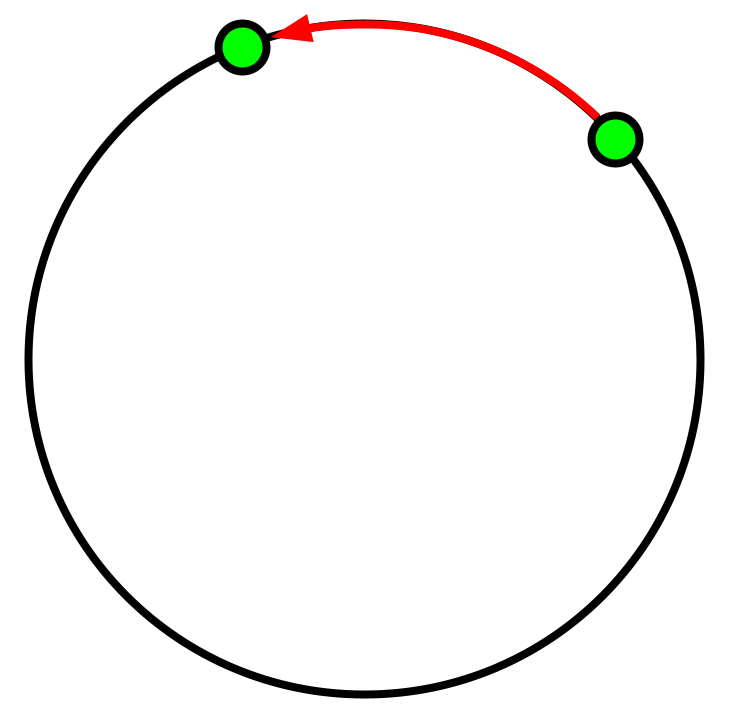
\includegraphics[width=0.3\textwidth]{Images/Chap0/Circle Metric.png}
  \end{center}
  \caption{Given two points, ($p_1$ to the right), $d$ is defined as the counter-clockwise angle from $p_1$ to $p_2$}
\end{wrapfigure}

Not all metric spaces are on the set $\R^2$, or even $\R$ for that matter. Consider the set $\mathbb{S}$, all the points on a circle. You may think of $\mathbb{S}$ as being all the points $(x,y)\in\R^2$ satisfying $x^2=y^2=1$. Given two points $p_1,p_2\in\mathbb{S}$, we can define a function $d(p_1,p_2)$ as being the angle in radians needed to travel counter-clockwise from $p_1$ to $p_2$. How might we explicitly write out this function?\\

Let's define $\mathbb{S}$ as being all the points $(x,y)\in\R^2$ satisfying $x^2=y^2=1$. Also, let $p_1=(x_1,y_1)$ and $p_2=(x_2,y_2)$. From basic trigonometry, we know the angle made with $p_1$ and the $x-$axis is $\arctan(y_1/x_1)$. From this we can deduce that the angle made between the two points is $\arctan(y_2/x_2)-\arctan(y_1/x_1)$. 

\begin{exercise}
    Show (with a counterexample) why $\arctan(y_2/x_2)-\arctan(y_1/x_1)$ is NOT a metric on $\mathbb{S}$.
\end{exercise}

\begin{exercise}
    Is it possible to alter our function slightly to create a metric? Or is there some critical issue with rotations about a circle?
\end{exercise}

Given any nonempty set $A$, we can create a ``trivial'' metric. Given $a,b\in A$, we have

\begin{equation}
d(a,b) = 
\left\{
    \begin{array}{lr}
        0, & \text{if } a=b\\
        1, & \text{otherwise }
    \end{array}
\right. 
\end{equation}

\begin{exercise}
    Prove that this forms a metric on any nonempty set $A$.
\end{exercise}

\subsection{Measures}

By defining a metric, we created a mathematical structure that describes the mapping of two objects to a positive number (or zero). Now, we will want to introduce a similar class of functions that maps a single object to a positive number. Before, our goal was to generalize our idea of distance (between elements), but now we want to generalize measuring the size of said objects, in particular, sets. \\

Cardinality is convenient for finite sets; simply count the number of elements in the set. But for infinite sets, cardinality is no longer very descriptive. For instance, when considering the intervals $[0,1]$ and $[0,2]$---all the real numbers between $0$ and $1$ and between $0$ and $2$ respectively---we see that $\#([0,1])=\#([0,2])$. This shows that the number of real numbers between $0$ and $1$, inclusive, is equal to the number of reals between $0$ and $2$. On an intuitive note, this feels absurd! The interval $[0,1]$ is entirely contained within the interval $[0,2]$. If we were to consider the lengths of these sets when graphed on the number line, the second would be twice as large as the first. Perhaps we would like to generalize this to allow us to find the length of any subset of $\R$. Regardless of how we define our function that measures these sets, there are a few things we want to ensure. 

\begin{itemize}
    \item The measure of a set that is empty should be $0$.
    \item Otherwise, the measure of a set should be positive.
    \item If a set is contained within another, the larger one should have a measure at least as large as the smaller.
    \item By combining disjoint sets (those that do not share any elements in common), their measures should add.
\end{itemize}

Like we did with metrics, these conditions will become our axioms for a \textbf{measure}. \\

Before establishing this definition, there is one more thing we must discuss. Since we want our definition of a measure to allow for countable unions of sets, we must make sure doing so is defined within our set of reference. We will define a special kind of algebraic structure that preserves this

\begin{definition}[$\sigma$-algebra]
    Given some set $X$ and its power set $\mathcal{P}(X)$, a set $\Sigma\subseteq \mathcal{P}(X)$ is a $\sigma$-algebra if
        \begin{itemize}
            \item $X \subseteq \Sigma$
            \item $A\in\Sigma \implies X / A\in\Sigma$
            \item $A_i\subseteq\Sigma \implies \bigcup_i A_i\subseteq \Sigma$
        \end{itemize}
\end{definition} 

This means 
\\

Based on our earlier discussion, here is our formal definition of a measure:\\

\begin{definition}[Measure]
    Given some $\sigma$-algebra $\Sigma$, a function $\mu$ from $\Sigma$ to $\R_\infty$ is a \textbf{measure} if
        \begin{itemize}
            \item $\mu(\varnothing)=0$
            \item For any $x\in\Sigma$, $\mu(x)\geq0$
            \item Given $x_1,x_2,x_3,\cdots$, a countable collection of pairwise disjoint sets in $\Sigma$, $\mu\left(x_1\cup x_2\cup\cdots\right)=\mu(x_1)+\mu(x_2)+\cdots$
        \end{itemize}
\end{definition} \index{Measure}
We refer to the set $\R_\infty$, sometimes written as $\R\cup\{\infty\}$; it is the set of real numbers, along with a symbol to represent infinite values. This is because some sets ought to have an infinite measure. The value of $\infty$ works as expected in the sense that adding it to any other value still yields $\infty$.\\

The first two axioms in our definition are somewhat self-explanatory. Just like how we created a zero-rule for metrics, we have a rule for measures that guarantees an image of $0$, regardless of the function or algebra. Moreover, measures have a similar structure to metrics in the sense that the results are 

Then give a brief overview of Lebesgue measure.\\

Give formal definition of trivial measure and prove it is a measure.\\

Introduce some properties of measures in general.\\

Insert exercises.\\

Explain that not all sets are Lebesgue measurable and give sources for more research.\\

\section{Topology}

In a general sense, topology is the branch of mathematics concerned with geometric properties of objects that are preserved under continuous transformations. This usually leads to the cliche illustration that states mathematicians perceive donuts and coffee mugs as the same object. Our objects may be geometric, or they could be just defined as sets, such as subsets of $\R^2$. But when there does exist a continuous transformation from one to the other (implying the transformation may be done in both directions), then we consider the objects $\textbf{homeomorphic}\index{Homeomorphic}$ and we call the function/transformation itself a \textbf{homeomorphism}\index{Homeomorphism}.\\

\begin{figure}
    \centering
    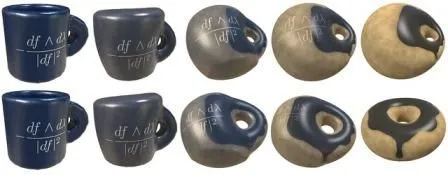
\includegraphics[width=0.5\linewidth]{Images/Chap0/0.4.1.png}
    \caption{Since there exists a continuous transformation from one object to the other, we consider the objects homeomorphic}
    \label{fig:donut-coffee}
\end{figure}

We will often talk about ``neighborhoods'' of points. The \textbf{$\e$-neighborhood} of a point in a metric space is the set of all points less than distance $\e$ of said point. For example, in $\R$ with the usual metric, the $2$-neighborhood of $3$ is all real numbers less than $2$ away from $3$: that is $(1,5)$ or $\{x\in\R\, :\, 1<x<5\}$. 

\begin{definition}[$\e$-neighborhood]
    The \textbf{$\e$-neighborhood} of $x$ in metric space $(X,d)$ is sometimes written as $V_\e(x)$. It is the set $\{y\in X \, :\, d(x,y)<\e\}$
\end{definition}\index{$\e$-neighborhood}

One of the fundamental topological characteristics we are concerned with is whether a set may be \textbf{open} or \textbf{closed}. First, for a set to be open, we require the set to have no boundary. Or in other words, no matter where you are inside the set, there

We define these terms as follows

\begin{wrapfigure}{l}{1.0\textwidth}
    
\includegraphics[width=0.9\linewidth]{Images/Chap0/0.4.2.png}
    \caption{Since there exists a continuous transformation from one object to the other, we consider the objects homeomorphic}
    \label{fig:donut-coffee}
\end{wrapfigure}

\begin{definition}[Open Set]
A set $X$ is \textbf{open} if for any point $x\in X$, there exists some $\e$ such that $V_\e(x)\subseteq X$. Or in other words, for all points in $X$, there exists an epsilon-neighborhood that is completely contained within $X$.     
\end{definition}\index{Open set}





\section*{Exercises}
\setcounter{section}{5}

\begin{exercise}
  Let $A = \{1, 3, 5, 7, 9\}$ and $B = \{2, 4, 6, 8, 10\}$.
  Determine the following sets. \\
  (a) $A \cup B$ \quad
  (b) $A \cap B$ \quad
  (c) $A \setminus B$ \quad
  (d) $A \times B$
\end{exercise}

\begin{exercise}
  Let $A = \{1, 2, 3\}$, $B = \{2, 3, 4\}$ and $C = \{3, 4, 5\}$.
  Determine the following sets. \\
  (a) $A \cup B \cup C$ \quad
  (b) $A \cap B \cap C$ \quad
  (c) $(B \setminus A) \cap C$ \quad
  (d) $(A \times B) \times C$
\end{exercise}

\section*{Project: \textbf{Convex Functions}}
\setcounter{section}{6}

In high school geometry, you were likely introduced to the idea of convex polygons, that is a polygon whose internal angles each do not exceed $180^\circ$. Geometric shapes $R \subseteq \E^2$ in general may be convex if for any $x,y\in R$ and for any $t\in[0,1]$, it follows that $tx+(1-t)y\in R$ as well. Notice that we are treating $x$ and $y$ like vectors, which is pretty convenient in $\E^2\simeq \R^2$. The point $(a,b)$ multiplied by $t$ would simply be $(ta,tb)$. In essence, our definition means for a convex shape, if we were to draw a line connecting $x$ and $y$, the entire line will remain inside $R$. \\

We may generalize this to any vector space (do not worry too much about us not introducing a definition of vector space, that is not as important here). We may say that for any vector space $S$ (which we may treat like a set), a set $C\subseteq S$ is convex if for all $x,y\in C$ and $t\in[0,1]$, $(1-t)x+ty\in C$.

\begin{example}[A region in $\R^2$]
    The unit square $[0,1]^2$ is convex
    \begin{proof}
        Let $P_1=(x_1,y_1)$ and $P_2=(x_2,y_2)$ be 2 points on or inside the unit square. This means that $x_1,y_1,x_2,y_2\in[0,1]$. Any point along the line segment connecting the two points may be described as \\$((1-t)x_1+tx_2,\ (1-t)y_1+ty_2)$ with $t\in[0,1]$. To show the unit square is convex, we must show $(1-t)x_1+tx_2\in[0,1]$ and $(1-t)y_1+ty_2\in[0,1]$. These two are identical so it is sufficient to just show the first.\\

        Since $t\in[0,1]$, either $t\in[0,\frac{1}{2}]$ or $(1-t)\in[0,\frac{1}{2}]$. Without loss of generality, assume $t\in[0,\frac{1}{2}]$ which implies $(1-t)\in[\frac{1}{2},1]$. Then 
        
        Since $x_1,x_2\in[0,1]$, we know $x_2-x_1\in[-1,1]$. Call this quantity $X=x_2-x_1$. Then, $(1-t)x_1+tx_2 = x_1 + t(x_2-x_1)=x_1+tX$. 
    \end{proof}
\end{example}